
\section{Architectural Design} \label{sec:arch}



\subsection{Architectural Diagram}
\vspace*{0.5in}
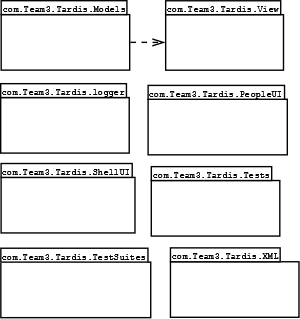
\includegraphics{diagrams/package_diagram}
\centerline {Figure 1: Package diagram}
\vspace*{0.2in}

Our system is designed with extensibility and scalability in mind.  We are taking great care in designing a framework which can be updated easily.  Many of the anticipated changes to our system in future phases will only require adding new types of data and changing the user presentation code to make use of these new data.  The framework we have designed will only require "plugging in" these new types of data without refactoring the logic that allows the user to view and manipulate the entered data, retrieves and updates the save file, etc.  There are four basic, logical components of the system: the Controller, the Models, the Views, and the Util.

\begin{itemize}

\item {\bf Controller}: The main controller that runs the tardis task manager.

\item {\bf Models}: Reader and Writer methods.

\item {\bf Views}: Display the output in one of four views.

\item {\bf Util} : Logger and input validators

\end{itemize}



\subsection{Subsystem Interface Specifications}

Specification of the software interfaces between the subsystems,
i.e. specific messages (or function calls) that are exchanged by the subsystems.
These are also often called ``Module Interface Specifications''.
Description of the parameters to be passed into these function calls in order to have a service fulfilled,
including valid and invalid ranges of values.
Each subsystem interface must be presented in a separate subsection.
